\section{DOCUMENTATION}
As this project integrates different kinds of elements and software modules and all the design would be used for next subjects, it was decided that some of the efforts were going to be allocated on generating 
good documentation of the code.

To approach this, doxygen\cite{DoxygenGettingstarted} was used. Doxygen defines both the standard and an application to generate documentation in a Javadoc style in both HTML and LaTex documents.

All the documentation in the code was defined following the doxygen specifications. Lastly, a Doxyfile configuration file is generated considering the needs of the documentation. This created the documentation files 
but two problems were observed:
\begin{enumerate}
    \item The default HTML documentation feels old, so a open style for Doxygen called "doxygen-awesome-css"\cite{jotheprodoxygenawesomecss} was used. This led to a much clean documentation as in the \autoref{fig:doxyStyle}.
    
    \begin{figure}[H]
        \centering
        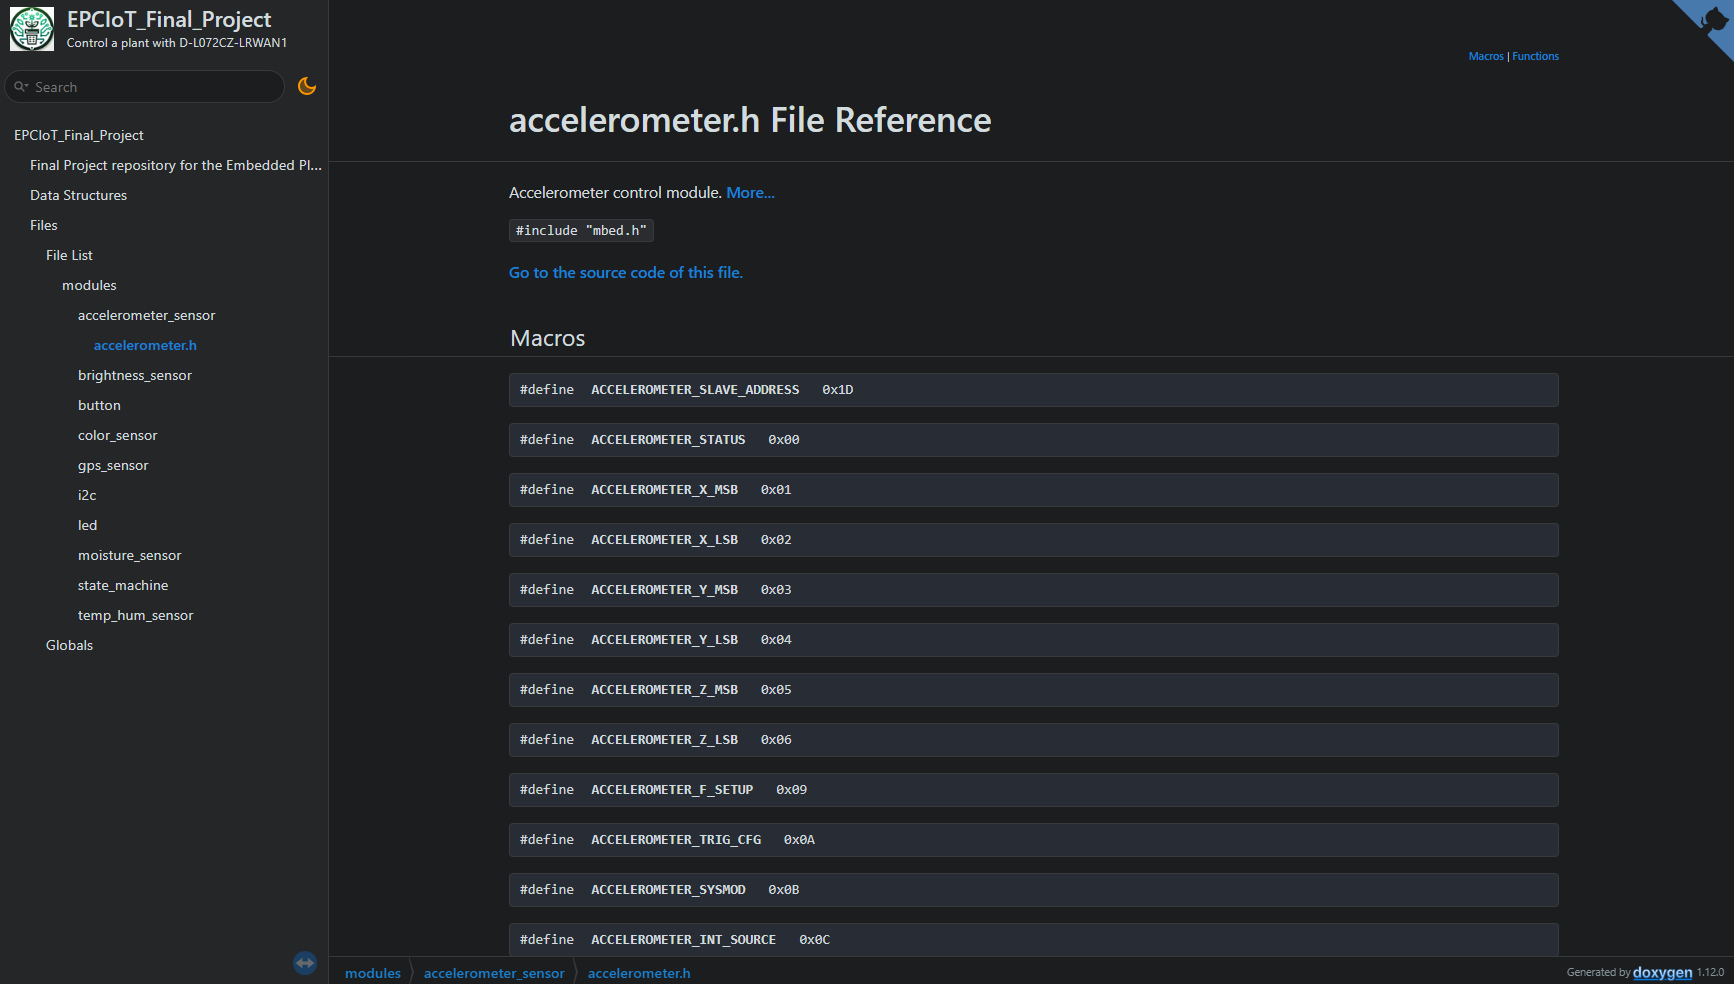
\includegraphics[width=0.8\textwidth]{images/8/doxy.png}
        \caption{Final documentation with the modified Doxygen}
        \label{fig:doxyStyle}
    \end{figure}

    \item As more functionalities were being added, the documentation needed to be re-generated. To solve this, a GitHub workflow was configured to auto-generate and auto-publish the generated HTML with an action in a branch of the repository. With GitHub pages, 
    the automatic deployment was configured.\newline The final result is available here: \url{https://ryvenkappa.github.io/EPCIoT_Final_Project/}
\end{enumerate}
